
\paragraph{Experiment 1}
We wish to solve the advection-diffusion problem presented in 
Section~\ref{ss:advdiff}:
\begin{equation}
\rho C_p u \frac{dT}{dx} - k \frac{d^2T}{dx^2} = f \qquad \text{in} \quad [0,L_x]
\end{equation}
with the boundary conditions $T(x=0)=0$ and $T(x=L_x)=0$.

The domain is characterised by $L_x=1$, and since $L_y$ is irrelevant it is set to $L_x/10$.
We further set $nelx=10$, $f=1$, $\rho=1$, $C_p=1$, $u=1$.
We will consider three values of the Peclet number: 0.25, 1 and 5.
From these values we can compute the corresponding heat conductivity value $k$.
Linear elements are used.

As $Pe$ increases, a sharp gradient, sometimes called a boundary layer,
develops at the right end of the domain. For high $Pe$ values, the solution shows 
spurious node to node oscillations, failing to capture the highly nonlinear change. This oscillatory
behavior is seen for $Pe>1$ (see Donea \& Huerta \cite{dohu03}).

\begin{center}
\includegraphics[width=5cm]{python_codes/fieldstone_65/results/solution1.pdf}
\includegraphics[width=5cm]{python_codes/fieldstone_65/results/solution2.pdf}
\includegraphics[width=5cm]{python_codes/fieldstone_65/results/solution3.pdf}\\
\includegraphics[width=5cm]{python_codes/fieldstone_65/results/T1.pdf}
\includegraphics[width=5cm]{python_codes/fieldstone_65/results/T2.pdf}
\includegraphics[width=5cm]{python_codes/fieldstone_65/results/T3.pdf}\\
{\captionfont Left to right: $Pe$=0.25, $Pe$=1, $Pe$=5}
\end{center}

Finally we see that we recover identical results as in Donea \& Huerta \cite{dohu03}:

\begin{center}
\includegraphics[width=8.6cm]{python_codes/fieldstone_65/images/dohu}
\end{center}

If we now use the artificial diffusion presented in Section~\ref{ss:supg}, we have
\[
\tilde{\kappa}=\beta \kappa Pe = \beta \frac{k}{\rho C_p} Pe
\]
with 
\[
\beta=\coth(Pe)-\frac{1}{Pe}
\]
which yields:
\[
\tilde{k} = \tilde{\kappa} \rho_0 C_p 
\]
and the code solves the following equation
\begin{equation}
\rho C_p u \frac{dT}{dx} - (k + \tilde{k})\frac{d^2T}{dx^2} = f \qquad \text{in} \quad [0,L_x]
\end{equation}


We observe that this approach recovers the analytical solution exactly:
\begin{center}
\includegraphics[width=5cm]{python_codes/fieldstone_65/results/artdiff/T1.pdf}
\includegraphics[width=5cm]{python_codes/fieldstone_65/results/artdiff/T2.pdf}
\includegraphics[width=5cm]{python_codes/fieldstone_65/results/artdiff/T3.pdf}\\
{\captionfont Left to right: $Pe$=0.25, $Pe$=1, $Pe$=5}
\end{center}

If one now uses 'full upwinding', i.e. $\beta=1$, we see that the scheme is 
overly dissipative (i.e. overly diffusive):

\begin{center}
\includegraphics[width=5cm]{python_codes/fieldstone_65/results/artdiff1/T1.pdf}
\includegraphics[width=5cm]{python_codes/fieldstone_65/results/artdiff1/T2.pdf}
\includegraphics[width=5cm]{python_codes/fieldstone_65/results/artdiff1/T3.pdf}\\
{\captionfont Left to right: $Pe$=0.25, $Pe$=1, $Pe$=5}
\end{center}

%..................................................................................
\paragraph{Experiment 2 - advection skew to the mesh}

The domain is a unit square. Resolution is $10\times10$ linear elements.

\begin{center}
\includegraphics[width=7cm]{python_codes/fieldstone_65/images/setup}
\includegraphics[width=7cm]{python_codes/fieldstone_65/results/exp2/vel}\\
{\captionfont Left: Taken from \cite{dohu03}. In our code we replace $u$ by the 
temperature $T$. Right: prescribed velocity field.}
\end{center}

\begin{remark}
On page 75 of \cite{dohu03} the authors state that 
"the diffusivity coefficient is taken to be $10^{-4}$ , 
corresponding to a mesh Peclet number of $10^4$. 
Given that $Pe=u h/2\kappa$ and h=0.1, this statement makes no sense.
I have therefore chosen $Pe=10^4$ and then 
$\kappa=uh/2Pe = 5\cdot10^{-6}$.
\end{remark}

The norm of the velocity vector $\vec{\upnu}$ is $|\vec{\upnu}|=1$. 
Since the Peclet number is so high, we have 
\[
\tau = \frac{h}{2 u_0} \left( \coth (Pe) -\frac{1}{Pe} \right) \rightarrow 
\frac{h}{2 u_0} 
\]


\begin{center}
\includegraphics[width=15cm]{python_codes/fieldstone_65/results/exp2/Temps}\\
\includegraphics[width=15cm]{python_codes/fieldstone_65/results/exp2/Temps2}\\
\includegraphics[width=15cm]{python_codes/fieldstone_65/images/exp2}\\
{\captionfont Left to right: Standard Galerkin method, artificial diffusion, SUPG. 
Bottom row taken from \cite{dohu03}. }
\end{center}



